\chapter*{Introducción}
\addcontentsline{toc}{chapter}{Introducción}

% =====================Estilo de página================================
\pagestyle{fancy}
\fancyhf{} % clear all header fields
\fancyhead[LE]{\nouppercase{\textbf{Introducción} \hfill}}
\fancyhead[RO]{\nouppercase{\hfill \textbf{Introducción}}}
\fancyfoot[LE]{\nouppercase{\thepage \hfill {Pressure Distribution Inside Nucleons in a
Tsallis-MIT Bag Model}}}
\fancyfoot[RO]{\nouppercase{{Pressure Distribution Inside Nucleons in a
Tsallis-MIT Bag Model} \hfill \thepage}}
% =====================================================================

% 12 345.678 90                     \num{12345,67890} \\
% 0.3 ×1045                         \num{.3e45} \\
% 1 ±2i                             \complexnum{1+-2i}
% 1.654 ×2.34 ×3.430                \numproduct{1.654 x 2.34 x 3.430}
% kg m s−1                          \unit{kg.m.s^{-1}}
% kg m s−1                          \unit{\kilogram\metre\per\second} 
% kg m/s                            \unit[per-mode = symbol]{\kilogram\metre\per\second}
% kg m/(A s)                        \unit[per-mode = symbol]{\kilogram\metre\per\ampere\per\second}
% \qty{10}{cm}

% \num{1.2304} \unit{\candela}
% \Gls{maths}

Entender la estructura interna de los hadrones es fundamental para descifrar las interacciones fuertes descritas por la \gls{qcd}. Este conocimiento no solo es crucial para la física de partículas, sino que también tiene implicaciones en la comprensión de la materia en condiciones extremas, como las que existieron en los primeros momentos del universo. Según el modelo de \gls{qcd}, las partículas hadrónicas están compuestas por quarks, los cuales permanecen confinados dentro de los hadrones. Este confinamiento es una de las características fundamentales de la \gls{qcd} y explica por qué no se han observado quarks libres en la naturaleza.

% Renombrando las figuras
\renewcommand{\figurename}{Fig.}

% \begin{wrapfigure}{r}{1\textwidth}
% \centering
% 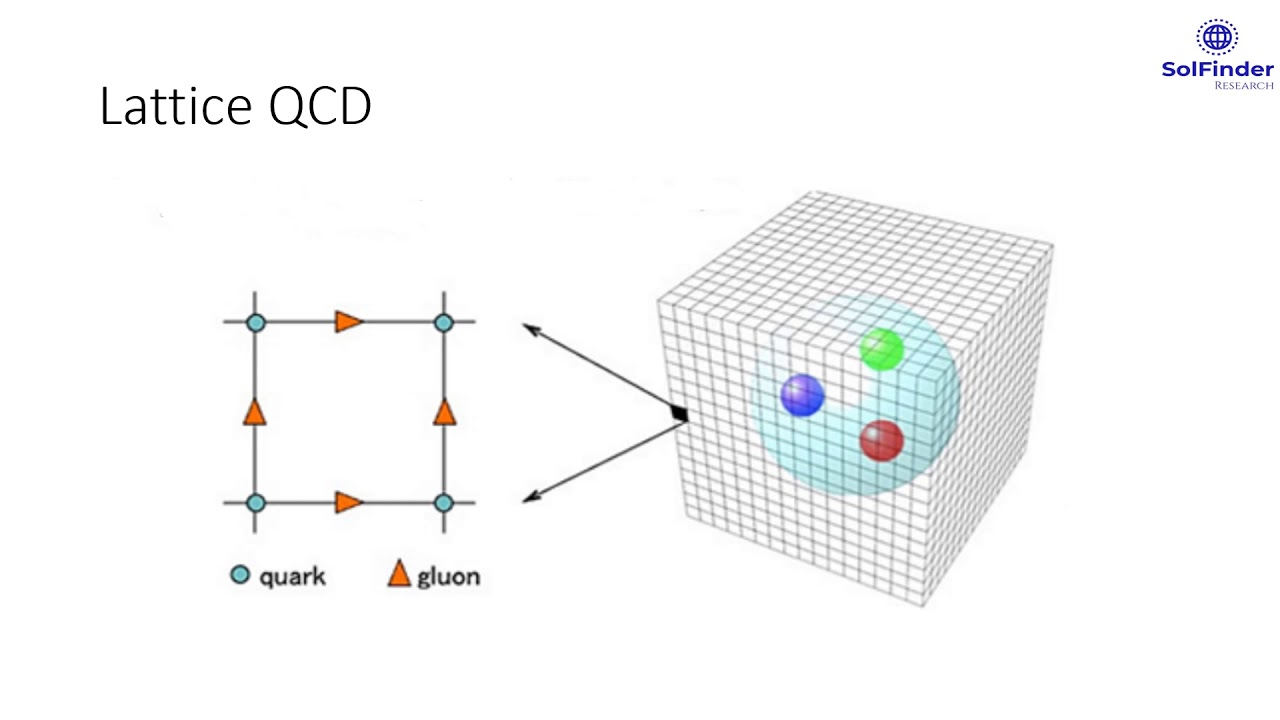
\includegraphics[width=1\textwidth]{./Images/LQCD.jpg}
% \caption[Red LQCD]{\emph{Diagrama de una red tipo LQCD, donde los nodos representan quarks y las aristas simbolizan campos gluónicos.}}
% \label{fig: LQCD}
% \end{wrapfigure}

\begin{figure}[h]
    \centering
    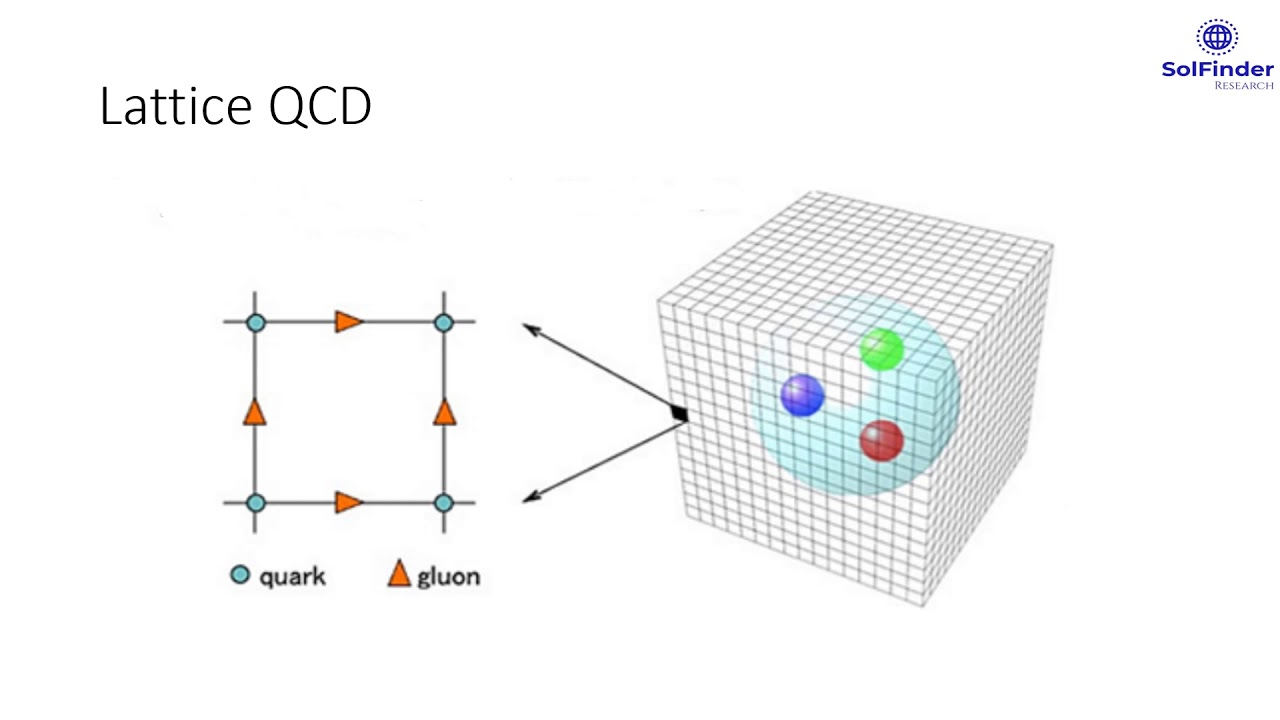
\includegraphics[width=0.8\textwidth]{./Images/LQCD.jpg}
    \caption[Red LQCD]{\emph{Diagrama de una red tipo LQCD, donde los nodos representan quarks y las aristas simbolizan campos gluónicos.} Fuente: Adaptado de Autor (Año).}
    \label{fig:LQCD }
\end{figure}

A lo largo de los años, se han propuesto diversos modelos fenomenológicos para describir la estructura del protón. Entre ellos destacan los modelos de cuerdas \cite{Artru1974, Andersson_1983}, que representan hadrones como cuerdas oscilantes; los modelos de bolsa \cite{AIHPA_1968__8_2_163_0,DeTar_1983}, que describen quarks confinados en una cavidad; y los modelos de valones \cite{Hwa_1981}. Cada uno de estos enfoques ofrece una perspectiva única sobre la naturaleza de los hadrones, pero todos enfrentan limitaciones al tratar de capturar la complejidad de las interacciones no lineales entre quarks y gluones.

Para explorar la física de la materia quark, se han desarrollado técnicas avanzadas que permiten estudiar estas interacciones. Una de ellas es la \gls{lqcd}, que utiliza simulaciones numéricas en redes espacio-temporales. Sin embargo, la complejidad de estos cálculos, que involucran millones de nodos, lleva a un problema conocido como \emph{el problema del signo}. Este problema surge en simulaciones Monte Carlo, donde los pesos de las configuraciones cuánticas pueden volverse negativos o incluso complejos, imposibilitando su interpretación como probabilidades clásicas %\cite{SignProblemReference}.

Recientemente, la colaboración \gls{hal-qcd} ha utilizado técnicas de \gls{lqcd} para realizar cálculos de vanguardia en el estudio de interacciones fuertes entre hadrones \cite{Iritani_2019,Hatsuda_2017}. Sus resultados, que describen sistemas protón-neutrón y protón-hiperón, han sido comparados con datos experimentales publicados por la colaboración \gls{alice} \cite{Collaboration2020, Collaboration2021}. Estos avances han sentado las bases para el desarrollo de modelos fenomenológicos más simples, como el que proponemos en este trabajo.

\begin{wrapfigure}{l}{0.45\textwidth}
    \centering
    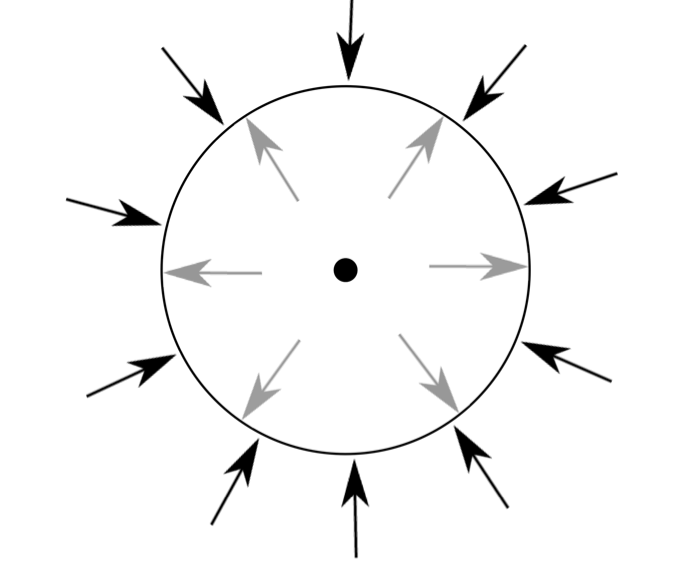
\includegraphics[width=0.4\textwidth]{./Images/Bag model.png}
    \caption[Diagrama de bolsa]{\emph{Diagrama que ilustra el modelo de bolsa. En el interior, la presión es generada por un plasma de quarks y gluones, mientras que la presión externa mantiene confinados estos componentes dentro del hadrón.} Fuente: Adaptado de Autor (Año).}
    \label{fig:Bolsa }
\end{wrapfigure}

En este trabajo, proponemos un modelo basado en el modelo de bolsa del \gls{mit} \cite{Chodos_1974,Chodos1974a} y la estadística no extensiva de \Gls{tsallis}. A este modelo lo denominamos \gls{t-mitbm}. El modelo de bolsa del \gls{mit} describe hadrones como recipientes cerrados que contienen un mar de quarks y gluones, los cuales interactúan dentro de los límites del hadrón (ver Fig.~\ref{fig:Bolsa }). Sin embargo, este modelo tradicional no captura completamente las interacciones no lineales entre quarks y gluones. Aquí es donde la estadística de \Gls{tsallis}, una generalización de la estadística de \gls{bg} \cite{Tsallis1988,Beck_2003,Tsallis2009,Tsallis_2014,Tsallis_2009}, juega un papel crucial.

La estadística de \Gls{tsallis} introduce un parámetro $q$ que captura las interacciones entre quarks y gluones, simplificando la no linealidad inherente a estas interacciones. Este enfoque ha demostrado ser exitoso en la descripción de sistemas complejos en física de altas energías, desde colisiones electrón-positrón \cite{Bediaga_2000,Collaboration1984} hasta colisiones de iones pesados \cite{Saraswat_2018,Saraswat_2017}. En nuestro modelo, combinamos el modelo de bolsa del \gls{mit} con la estadística de \Gls{tsallis} para estimar la distribución de presión total dentro de los nucleones.

El objetivo principal de este trabajo es proponer un modelo fenomenológico que combine el modelo de bolsa del MIT con la estadística no extensiva de \Gls{tsallis} para estudiar la distribución de presión dentro de los nucleones. Comparamos nuestros resultados con la distribución de presión de quarks obtenida recientemente mediante técnicas de \gls{dvcs} \cite{Burkert_2018}. Estas técnicas, que involucran la dispersión de fotones virtuales de altas energías, han permitido medir la presión repulsiva de los quarks cerca del centro del protón y una presión de confinamiento a distancias mayores de $0.6$.

En los siguientes capítulos, describiremos en detalle el marco teórico del \gls{t-mitbm}, los resultados obtenidos y las comparaciones con datos experimentales. En el Capítulo \ref{ch-BagModel}, explicamos el modelo de bolsa y sus limitaciones. En el Capítulo \ref{ch-Tsallis}, presentamos la estadística no extensiva de \Gls{tsallis} y su aplicación al plasma de quarks y gluones. En el Capítulo 5, comparamos nuestros resultados con los datos experimentales de presión de quarks, y en el Capítulo 6, discutimos una posible interpretación física del parámetro de \Gls{tsallis} $q$. Finalmente, en el Capítulo 7, presentamos las conclusiones y perspectivas futuras de este trabajo.

\newpage

\thispagestyle{empty}